El proyecto sTGC Minería se compone de tres sistemas principales: disparo, detección y adquisición, como se ilustra en la Figura \ref{fig:sistema-completo}. Como se introdujo en la Sección \ref{sec:planteamiento}, el sistema de disparo \cite{Oyanadel2020SistemaSTGC} (ilustrado en azul),  está formado por dos detectores centelladores y una unidad de coincidencias que emite una señal digital de disparo (indicada en celeste) cuando un muon traspasa ambos detectores centelladores. Esta señal de disparo es necesaria para discriminar eventos captados por el detector sTGC y descartar interacciones procedentes de otras partículas cargadas que no sean muones. \gcnote{(Para discutir) Este sistema de deteccion ya se encuentra fabricado? Por que no se trata en este trabajo?}
	
Si bien los detectores centelladores presentes en el sistema de disparo son capaces de detectar exclusivamente el paso de muones, estos no son capaces de determinar la ubicación del vértice de interacción. Para cumplir con este requerimiento de localización, se utilizan los detectores complementarios al sistema de detección sTGC (ilustrados en verde en la Figura \ref{fig:sistema-completo}) \gcnote{revisar colores}, sistema que es capaz de determinar la ubicación de los vértices de interacción gracias a su tecnología de fabricación.
	
En este capítulo se detalla la forma y funcionamiento del sistema de detección, describiendo el prototipo de detector sTGC utilizado en sTGC Minería y describiendo también la interfaz de lectura ASD \gcnote{introdujiste ASD?} que lo sucede. \gcnote{Clarificar explicitamente si esto ya esta implementado o haras algo con esto en tu memoria.}Es necesario conocer las características de estas etapas, ya que determinan la cantidad y tipos de señales a leer en el sistema de adquisición de datos a ser diseñado en este proyecto de titulación.
	

\gcnote{Estudiar este sistema fue parte de tu memoria?}

	\begin{figure}[h]
		\centering
		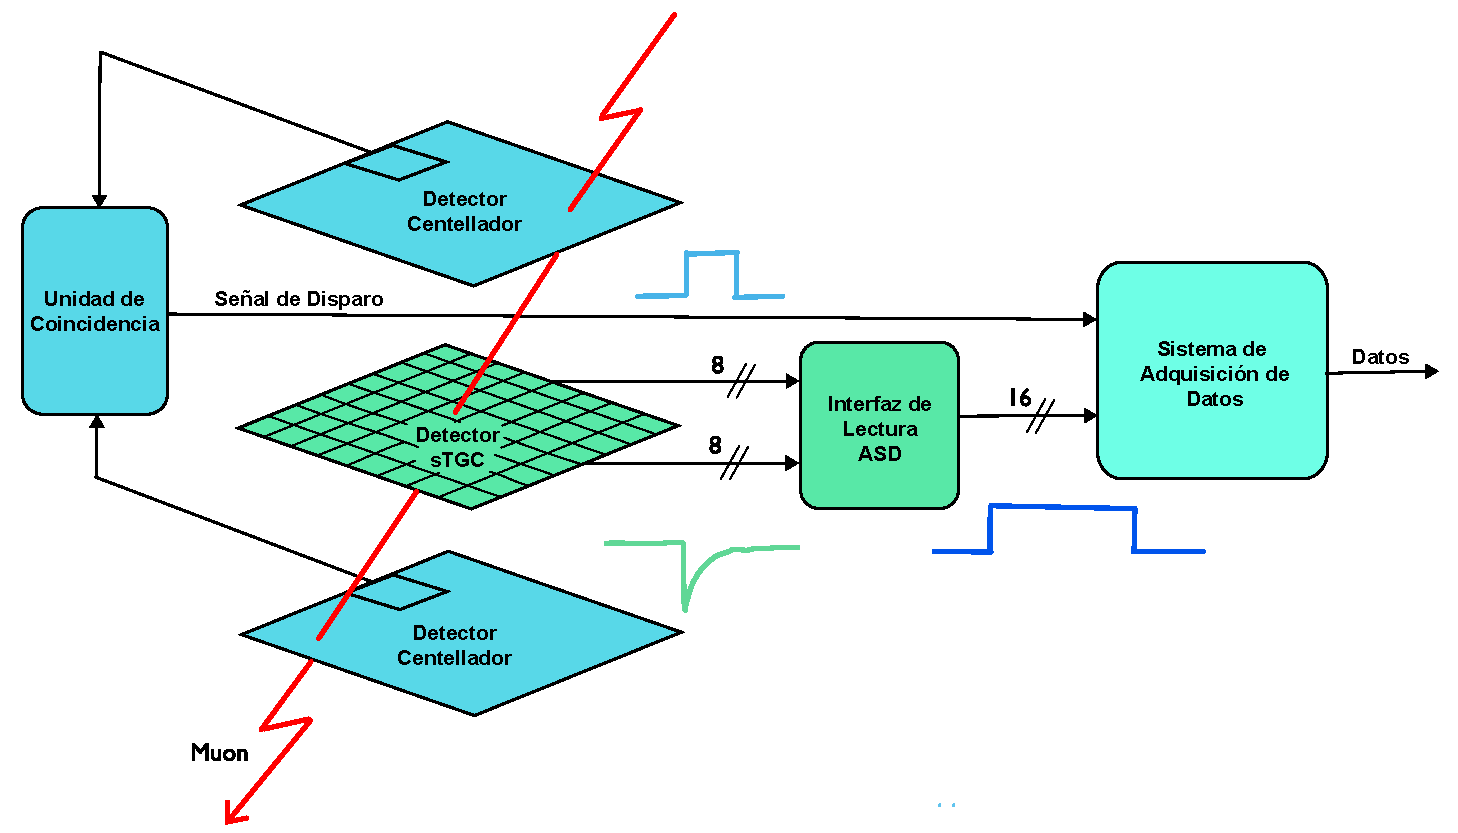
\includegraphics[scale=0.55]{sistema.pdf}
		\caption{Diagrama del sistema de muongrafía de terreno utilizando un solo detector.}
		\label{fig:sistema-completo}
	\end{figure}